
\section{DINÁMICA TRASLACIONAL}
\subsection{Arrastre y levantamiento}
\begin{frame}{DINÁMICA TRASLACIONAL}
\framesubtitle{Arrastre y levantamiento}
	La resistencia del aire se puede descomponer en las componentes x y y del movimiento y
nombrarlas como una fuerza de arrastre y una de levantamiento respectivamente.
	\begin{figure}[H]
      \centering
      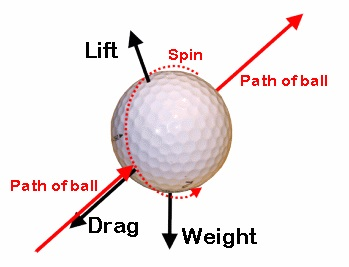
\includegraphics[scale = 0.5]{forces.jpg}
      \caption{Diagrama de cuerpo libre para una bola de golf\footnotemark{}.}
    \end{figure}
     \footnotetext{\bibentry{forces}.}
\end{frame}

%%%%%%%%%%%%%%%%%%%%%%%%%%%%%%%%%%%%%%%%%%%%%%%%%%%%%%%%%%%%%%%%%%%%%%%%

\subsection{Números de Reynolds}
\begin{frame}{DINÁMICA TRASLACIONAL}
\framesubtitle{Números de Reynolds}
	Depende del diametro del objeto de estudio ($D$), la viscocidad del fluido ($\mu$), la densidad del fluido ($\rho$) y la velocidad del fluido ($v$).
	\begin{equation}
		Re=\frac{\rho vD}{\mu}
	\end{equation}
    \begin{figure}[H]
      \centering
      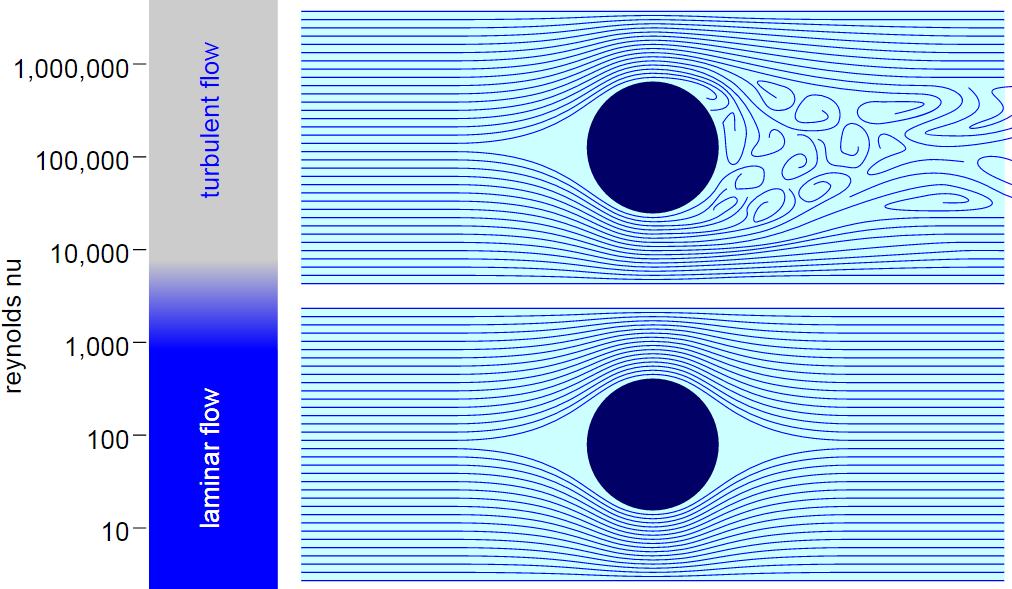
\includegraphics[scale = 0.25]{Flow-Regime.png}
      \caption{Comportamiento del fluido de acuerdo a los valores del número de Reynolds.\footnotemark{}.}
    \end{figure}
     \vspace{-1cm}\footnotetext{\bibentry{reynolds2}.}
   	\end{frame}
    
%%%%%%%%%%%%%%%%%%%%%%%%%%%%%%%%%%%%%%%%%%%%%%%%%%%%%%%%%%%%%%%%%%%%%

\subsection{Crisis de arrastre}
\begin{frame}{Dinámica traslacional}
\framesubtitle{Crisis de arrastre}
	Al analizar la gráfica de fuerza de arrastre contra número de Reynolds se obtiene un resultado algo contradictorio para la época.
	\begin{figure}[H]
      \centering
      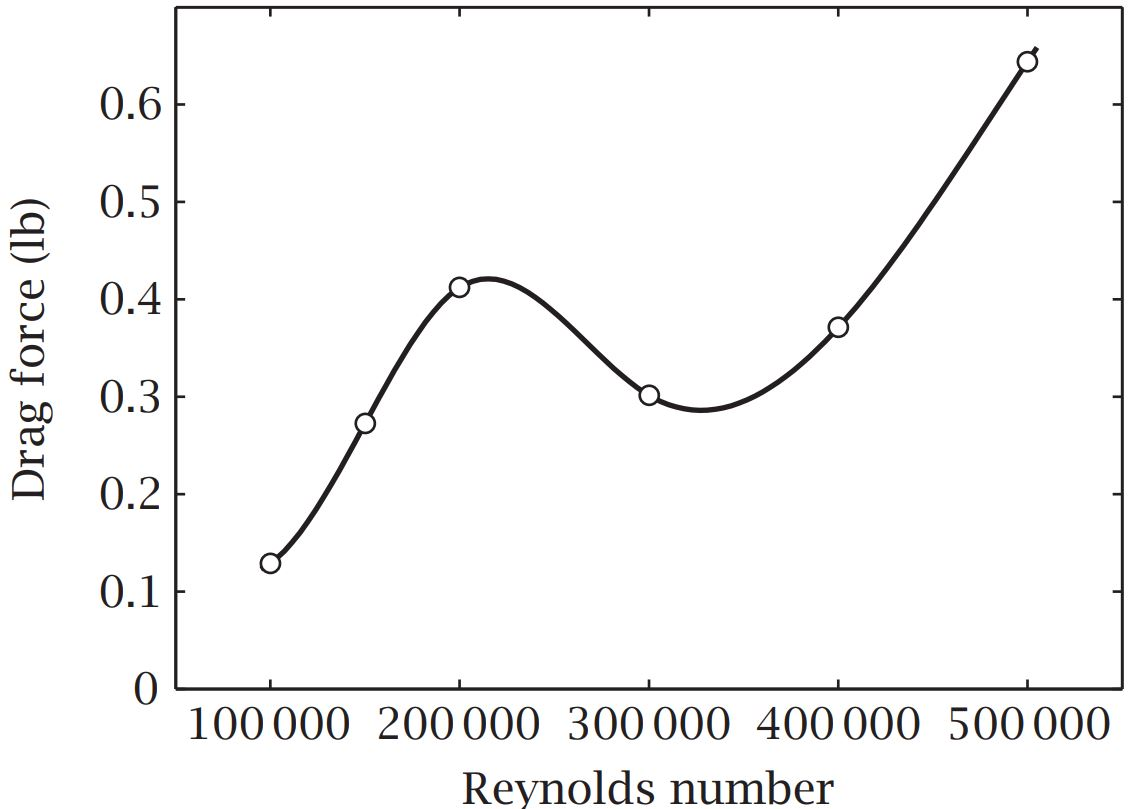
\includegraphics[scale = 0.2]{DragVSRey.JPG}
      \caption{Diagrama de las etapas del fluido al rededor de la bola.\footnotemark{}.}
    \end{figure}
     \footnotetext{\bibentry{golf-flight}.}
   \end{frame}
 %%%%%%%%%%%%%%%%%%%%%%%%%%%%%%%%%%%%%%%%%%%%%%%%%%
\begin{frame}{Dinámica traslacional}
\framesubtitle{Crisis de arrastre}
	\begin{figure}[H]
      \centering
      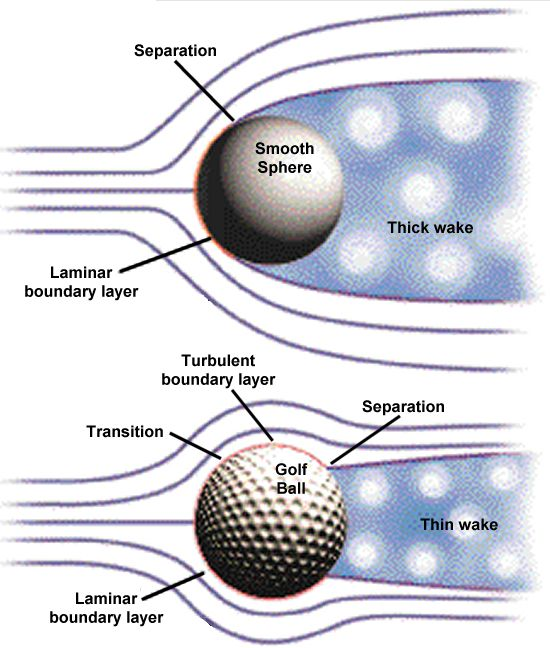
\includegraphics[scale = 0.2]{dimpled.jpg}
      \caption{Bola de golf vs bola suave.}
    \end{figure}
\end{frame}

%%%%%%%%%%%%%%%%%%%%%%%5
\begin{frame}{Dinámica traslacional}
\framesubtitle{Crisis de arrastre}
	\begin{figure}[H]
      \centering
      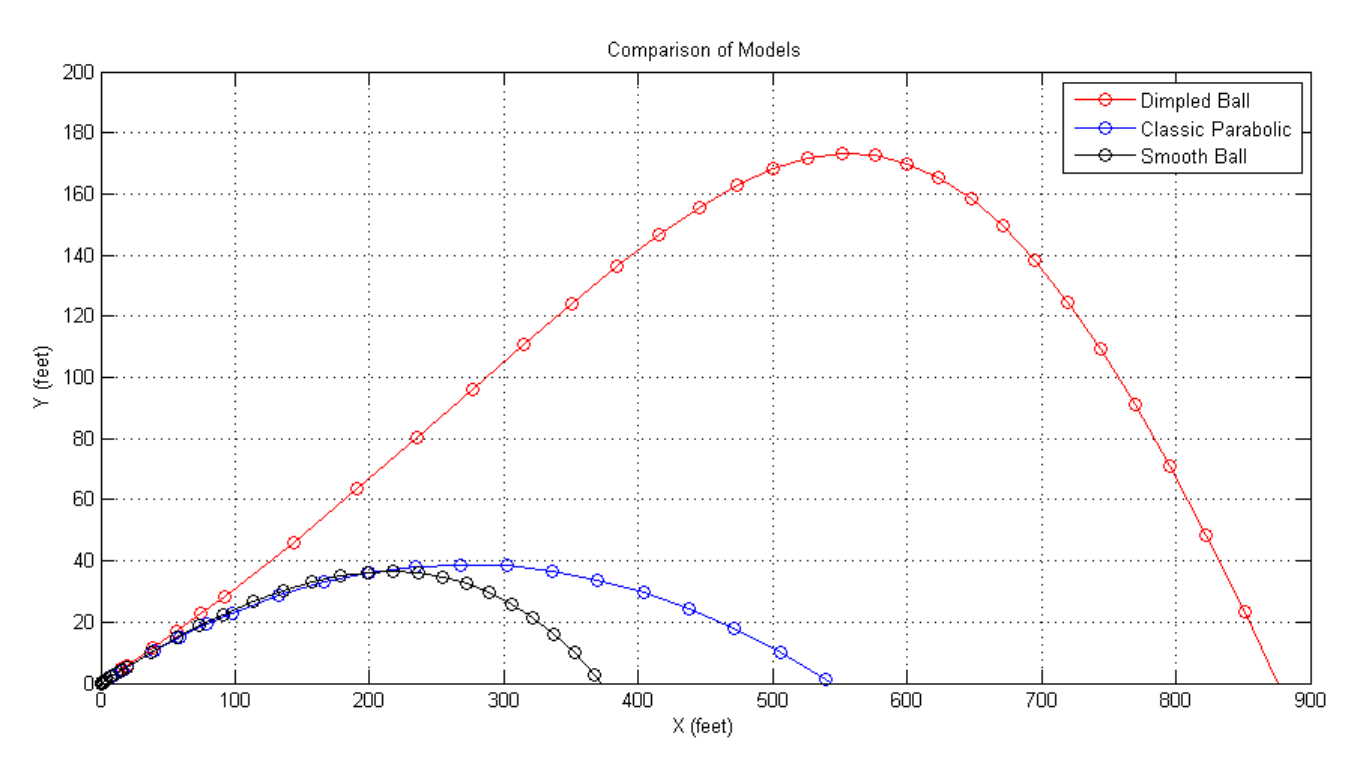
\includegraphics[scale = 0.2]{Comp.png}
      \caption{Bola de golf vs bola suave.}
    \end{figure}
\end{frame}
 %%%%%%%%%%%%%%%%%%%%%%%%%%%%%
 \subsection{Explicación de la crisis}
 \begin{frame}{DINÁMICA TRASLACIONAL}
 \framesubtitle{Explicación de la crisis}
 	\begin{itemize}
 	\item Turbulencia de la capa límite.
    \item Combinación de aire rápido y lento. 
    \item Separación de la capa límite.
    \item Reducción de la fuerza de arrastre
 	\end{itemize}
    \begin{figure}[H]
      \centering
      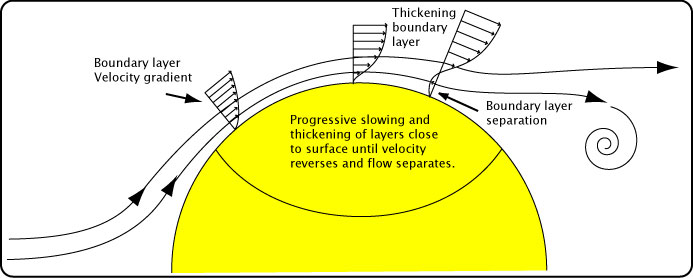
\includegraphics[scale = 0.3]{grad.jpg}
      \caption{Diagrama de cuerpo libre para una bola de golf\footnotemark{}.}
    \end{figure}
     \footnotetext{\bibentry{crisis}.}
 \end{frame}

%%%%%%%%%%%%%%%%%%%%%%%%%%%%%%%%%%%%%
 \subsection{Fuerzas ejercidas por el golfista}
 \begin{frame}{DINÁMICA TRASLACIONAL}
 \framesubtitle{Fuerzas ejercidas por el golfista}
 \textbf{- Reacción del piso:}
 	\begin{itemize}
 	\item $65\%$ del peso se encuentra sobre el pie trasero durante el backswing
    \item Transfieren rápidamente el peso de un pie a otro 
    \item El pico de mayor peso sobre el pie delantero se alcanza en la mitad del downswing
    \item Los jugadores con menos habilidades no transfieren tanto peso de un pie a otro y lo hacen de manera más lenta.
 	\end{itemize}
    \begin{figure}[H]
      \centering
      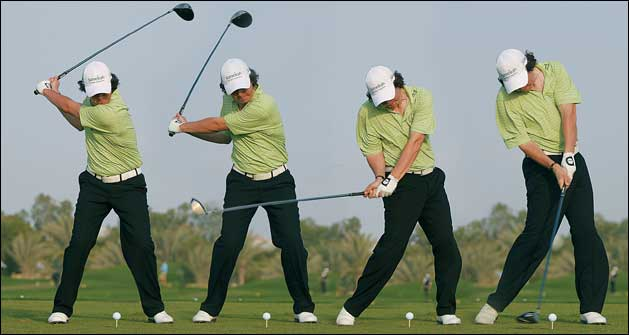
\includegraphics[scale = 0.25]{player.jpg}
      \caption{Jugador realizando un swing\footnotemark{}.}
     \end{figure}
     \vspace{-2cm}\footnotetext{\bibentry{player}.}
\end{frame}
%%%%%%%%%%%%%%%%%%%%%%%%%%%%%%%%%%%%%%
\begin{frame}{DINÁMICA TRASLACIONAL}
\framesubtitle{Fuerzas Musculares}
Los jugadores más avanzados utilizan los grades músculos de las piernas y las caderas para obtener más potencia, mientras que los que tienen menos habilidades requieren más fuerza en brazos y espalda.
\begin{figure}
  \centering
  \begin{subfigure}[H]{0.3\textwidth}
    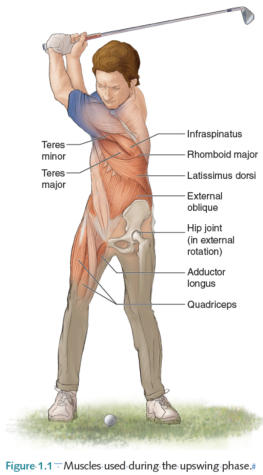
\includegraphics[scale = 0.25]{body1.jpg}
    \centering
    %\caption{Paisaje 1.}
  \end{subfigure}
  \hspace{-1cm} % Add desired spacing between images, e. g. ~, \quad, \qquad, \hfill etc (or a blank line to force the subfigure onto a new line)
  \begin{subfigure}[H]{0.3\textwidth}
    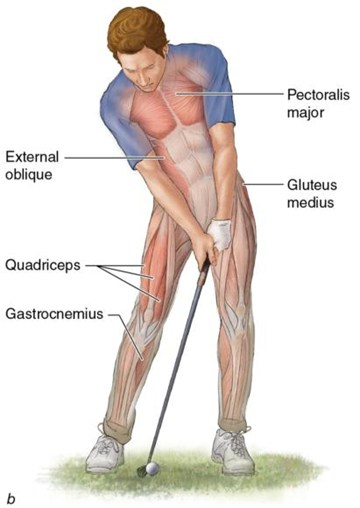
\includegraphics[scale = 0.25]{body2.jpg}
    \centering
    %\caption{}
  \end{subfigure} % a spacing can be put before caption
  \vspace{-2mm}
  \caption{Músculos utilizados durante un swing\footnotemark{}.}
\end{figure}
\footnotetext{\bibentry{body}}
\end{frame}


